%\part*{Lezione 15/04/2021}
\subsection{LUNA}\esperimento{LUNA}\label{sec-LUNA}
Discutiamo in questa sezione il \textit{Laboratory for Underground Nuclear Astrophysics} detto LUNA.

\paragraph{Un po' di storia} 
I lavori per l'esperimento LUNA iniziarono nel 1990 insieme a quelli al Gran Sasso ed è tuttora operativo.
\begin{enumerate}
	\item LUNA I\footnote{Fu impiegato un acceleratore \textit{\vir{home made}}, progetto di laurea di uno studente, che cosisteva di un Van de Graaff a 50 kV. Il fascio aveva uno \textit{spread} $<20$ eV (molto piccolo) che peremetteva un'accurata determinanzione dell'energia delle particelle incidenti e inoltre il voltaggio era noto meglio di 1 parte su $\ord{-4}$.} dal 1994 al 2003.
	\item LUNA II dal 2000 al 2020.
	\item LUNA MV in progettazione.
\end{enumerate}

\subsubsection{LUNA I}\esperimento{LUNA!LUNA I}\label{sec-LUNA-I}
\paragraph{La prima reazione} Nell'esperimento LUNA I si studiò per prima la reazione\footnote{Reazione $pp$I, guarda Figura \ref{0318_solnu}.}:
$$\ce{^3He} + \ce{^3He} \to \ce{^4He} + 2p$$
dove un $\ce{^3He}$ cosisteva in un fascio con una corrente pari a 300 $\mu$A e l'altro in una targhetta gassosa posta nella camera di interazione a una pressione\footnote{Da una versione a quella successiva si è migliorato anche questo settaggio.} di $0.5$ mbar. Un \textit{beam dump}, anch'esso collocato nella camera di interazione, bloccava il fascio e permetteva, tramite la misura della variazione di temperatura, di stimare la \textit{beam current} con una precisione del 3\%\footnote{Per ottenere questa precisione era stato posto nella camera anche un calorimetro che tenesse conto dell'effetto di ionizzazione dovuto al passagggio del fascio attraverso il gas.}.
\complementi{l'ipotesi di Fowler} %
\\
\noindent Fu scelta questa reazione non solo perché presente nella $pp$I\index{Catena protone-protone@Catena protone-protone $pp$!e@$pp$I}, ma anche perché negli anni '90 era particolarmente discussa la questione dei neutrini solari e Fowler aveva supposto che la sezione d'urto di tale reazione fosse sottostimata a causa di una risonanza non osservata\footnote{Guarda la sezione \secrif{0325-sec-risnu} per l'ipotesi di Fowler.}. Prima di LUNA non si avevano acquisizioni per energie inferiori ai 26 keV e il picco di Gamow di tale reazione è $21 \pm 5$ keV; con LUNA I si raggiunsero $16.5$ keV misurando\footnote{Si avevano 2 eventi al mese.} una sezione d'urto pari a 20 fb$= 2\cdot \ord{-38}\unit{cm}^2$. Il rivelatore (composto da quattro $\Delta E$-$E$ \textit{particle detector}\footnote{La configurazione dei rivelatori $\Delta E -E$ consiste in due mezzi di diverso spessore posti in successione: $\Delta E$ si riferisce all'energia persa dal fascio nell'attraversamento del mezzo più sottile, mentre $E$ a quella scambianta con il mezzo più spesso, che \vir{frena} il fascio.}) permetteva di identificare evento per evento una regione in cui l'evento stesso si collocava, al fine di poter stimare il contributo dell'\textit{induced background}\index{ZZBackground@\textbf{Background}!induced@\textit{induced}}\footnote{Ovvero il fondo indotto dalla misura stessa.}: nel fascio era presente infatti una contaminazione di deuterio di circa $d/\ce{^3He}\sim 1\cdot\ord{-7} \div 5\cdot\ord{-6}$ e questa \vir{sporcava} la misura a causa della reazione $\ce{^3He}(d,p)\ce{^4He}$\footnote{La cui sezione d'urto è $\ord{6}$ volte maggiore di quella della reazione di interesse.}. In Figura \ref{0415_DEE} riportiamo i risultati della presa dati: si possono facilmente distinguere 2 regioni differenti. 


\begin{figure}[!h]
	\centering
	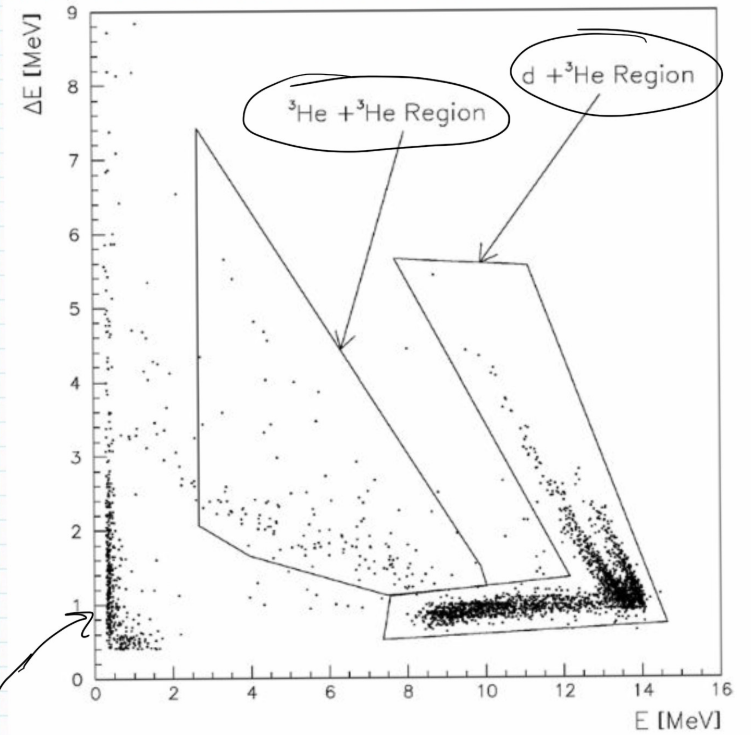
\includegraphics[scale=0.5]{Immagini/0415_DE-E.png}
	\caption{Dati dell'esperimento. Si riescono a identificare 2 regioni, una di interesse e l'altra di rumore. Si osserva anche una zona particolarmente popolata nelle basse energie lungo le ascisse che è dovuta al rumore elettronico indotto dal fascio.}
	\label{0415_DEE}
\end{figure}

\noindent Si osserva anche la presenza di un certo \textit{noise} sulle ascisse, che tuttavia non preoccupa dal momento che la regione di interesse è molto meno popolata.\\
Per energie inferiori ai $20.7$ keV le 2 regioni si sovrapponevano e non era più possibile distinguere tra fondo e misura di interesse, allora furono installati 2 rivelatori di protoni in successione e in coincidenza, dal momento che la reazione $\ce{^3He}(d,p)\ce{^4He}$ produce un solo protone e non due. Per avere un'idea di quanto fu ridotto il fondo si guardi la Figura \ref{0415_r1r2}.

\begin{figure}[!h]
	\centering
	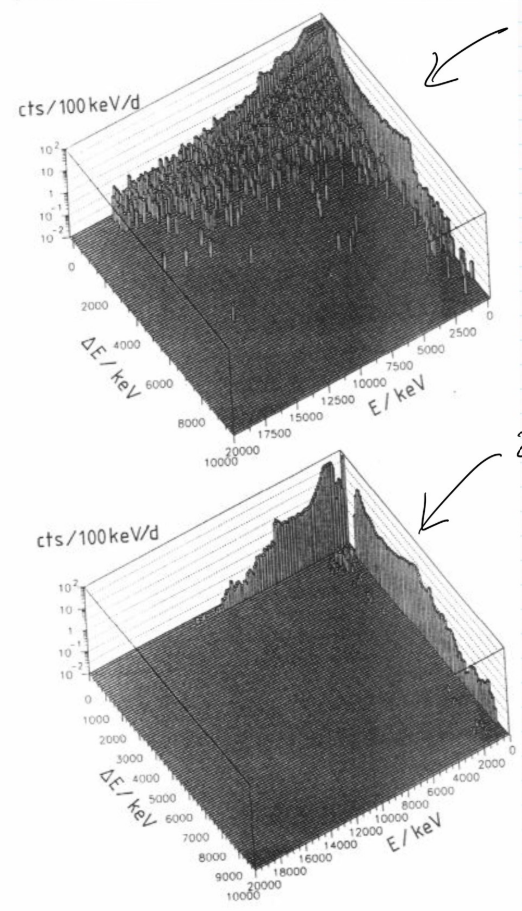
\includegraphics[scale=0.5]{Immagini/0415_riv12.png}
	\caption{Riduzione del fondo, sul piano $x-y$ vi è la matrice $\Delta E$-$E$, mentre sull'asse $z$ sono riportati i conteggi: in alto risultati con \textit{running time} di 16 giorni per un solo rivelatore a terra (presenza anche di raggi cosmici), in basso 2 rivelatori in coincidenza nel sottosuolo con \textit{runnig time} di 61 giorni.}
	\label{0415_r1r2}
\end{figure}

\noindent Si ottenne così i risultati per la sezione d'urto e il fattore astrofisico di Figura \ref{0415_sigma}. Notiamo che per basse energie il fattore astrofisco tende a crescere; ciò è dovuto non a una risonanza sotto soglia, ma dai risultati del fit sembrerebbe legato all'elettroscreening\index{elettroscreening}\footnote{Riguarda la sezione \secrif{0329-sec-screening}.}:
$$\frac{\sigma_{lab} (E)}{\sigma_{bare} (E)} \sim \exp{\ppc{\frac{\pi\eta U_e}{E}}}$$
Fu confutata così l'ipotesi di Fowler\complementi{l'ipotesi di Fowler} e non solo, si potè valutare anche l'effetto dell'elettroscreening\index{elettroscreening}.

\begin{figure}[!h]
	\centering
	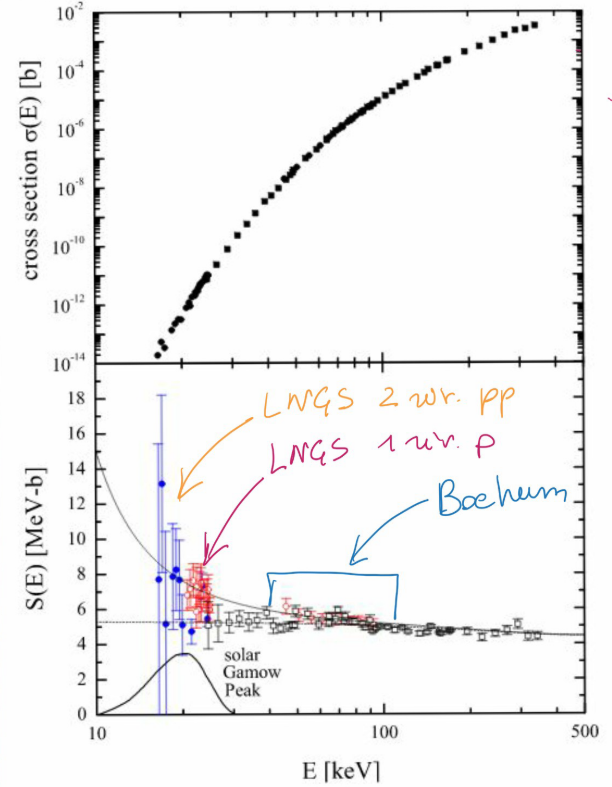
\includegraphics[scale=0.5]{Immagini/0415_sigma.png}
	\caption{Risultati degli esperimenti. In alto la sezione d'urto; in basso il fattore astrofisico: i cerchi blu pieni sono i risultati al Gran Sasso con rivelatori di protoni in coincidenza, i cerchi rossi vuoti per energie comprese tra 20 e 25 keV sono i dati LUNA I con un solo rivelatore di protoni, mentre per energie tra 45 e 92 keV (soglia in cui il segnale è maggiore del \textit{background)} sono i dati raccolti con lo stesso rivelatore ma a Bochum in Germania a terra. La \vir{risalita} del fattore astrofisico è dovuta all'elettroscreening\index{elettroscreening}.}
	\label{0415_sigma}
\end{figure}

\paragraph{Il problema dello screening} L'effetto di elettroscreening\index{elettroscreening} dato dal modello $U_e = 220$ eV non era compatibile con quello misurato $U_e\simeq (294 \pm 47)$ eV. Si iniziò quindi a studiare tale fenomeno. Fu scelta la reazione (precedentemente non di interesse):
$$d + \ce{^3He} \to \ce{^4He} + p$$
arrivando a energie inferiori a $4.2$ keV, come mostrato in Figura \ref{0415_escreen}. Nonostante l'accordo qualitativo, si ottenne così $U_e^{exp} \simeq (132\pm 9) $ eV, non compatibile con $U_e^{th}\equiv U_{ad} = 65$ eV.

\begin{figure}[!h]
	\centering
	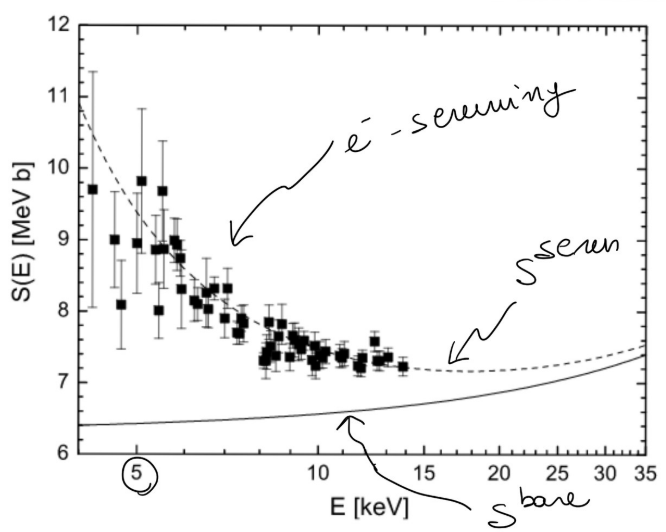
\includegraphics[scale=0.7]{Immagini/0415_SE.png}
	\caption{Dati di LUNA I per il fattore astrofisico: la linea continua rappresenta il modello senza schermo elettronico, la linea tratteggiata quello che ne tiene conto.}
	\label{0415_escreen}
\end{figure}
\noindent L'ultima reazione studiata in questo campo è:
$$p + d \to \ce{^3He} + \gamma$$
intorno al picco di Gamow. Questa reazione fa parte della catena $pp$\index{Catena protone-protone@Catena protone-protone $pp$}\footnote{Importante nelle proto-stelle: quando si raggiungono temperature $T\sim \ord{6}$ K il poco deuterio presente (dovuto all'arricchimento di popolazioni precedenti) può reagire $p+d$, innescando un $d$-\textit{burning} prima della catena $pp$. Questo comporta un rallentamento della contrazione e quindi un aumento della vita media della proto-stella: le sue caratteristiche (luminosità, temperatura,\dots) rimangono infatti \vir{congelate} fin quando dura il $d$-\textit{burning} e ciò avrà conseguenze su tali quantità all'innesco del H-\textit{burging} successivo.\complementi{Evoluzione protostellare}}, ma è l'unico canale aperto per cui non influisce sul conto dei neutrini solari. 
I \textit{range} di energie di interesse per questa reazione:
\begin{itemize}
	\item $1-2$ keV $\to$ $d$-\textit{burning} di proto-stelle.
	\item $\simeq 9$ keV $\to$ $d$-\textit{burning} del Sole.
	\item $\simeq 100$ keV $\to$ $pd$ della BBN\index{Big Bang Nucleosynthesis}.
\end{itemize}
LUNA I si concentrò sulle energie inferiori ai 100 keV e dovette ovviamente cambiare \textit{set-up} dal momento che l'interazione era differente (elettromagnetica): rivelatore ad alta efficienza (prendere più eventi possibile) e a largo angolo solido (ampio campo di osservazione). Fu impiegato il BGO%? Si tratta di un cristallo
 ($\ce{Bi_4}\ce{Ge_3}\ce{O_{12}}$)\index{BGO} come scintillatore, dotato di un'efficienza di circa 70\% e una risoluzione in $E\sim 8\%$.


\subsubsection{LUNA II}\label{sec-LUNAII}\esperimento{LUNA!LUNA II}
Nel 2000 LUNA II fu impiegato per lo studio della $pd$ della BBN (100 keV). Fu utilizzato un acceleratore commerciale a \textit{high current} (Cockcroft-Walton): 1 mA per H$^+$ e 500 $\mu$A per He$^+$ con un voltaggio pari a 400 kV, rimanendo stabile anche per 40 giorni di operatività. Furono costruite 2 linee di prese dati:
\begin{enumerate}
	\item[I] targhetta gassosa
	\item[II] targhetta solida
\end{enumerate}
Le reazioni studiate da LUNA II furono:
\begin{enumerate}
	\item $\ce{^3He(\alpha,\gamma)\ce{^7Be}}$, studio della BBN e della $pp$.
	\item $\ce{^{14}N(p,\gamma)^{15}O}$, studio biciclo CN-NO\footnote{Guarda la sezione}.%! INSERIRE SEZIONE
	\item $\ce{^{25}Mg(p,\gamma)^{26}Al}$, studio di altri cicli stellari.
	\item $pd$, studio della BBN. 
\end{enumerate}
Ricordiamo la Figura \ref{0315_astr2}, dove compaiono in rosso per basse energie i dati di LUNA I (Casella 2002) e per energie maggiori quelli di LUNA II.

\paragraph{Lo studio della $\mbox{he}\alpha$} Discutiamo adesso la reazione $\ce{^3He(\alpha,\gamma)\ce{^7Be}}$. Prima di LUNA erano stati sviluppati 2 metodi di misura:
\begin{enumerate}
	\item \textit{Prompt} $\gamma$ \textit{method}\index{misura di Be@Misura di $\ce{^3He(\alpha,\gamma)\ce{^7Be}}$!prompt g method@\textit{prompt} $\gamma$ \textit{method}} che si basa principalmente sulla misura dei fotoni prodotti. Da questo si era ottenuto:
	$$S(0) = (0.507 \pm 0.016) \unit{keVb}$$
	\item \textit{Activation method}\index{misura di Be@Misura di $\ce{^3He(\alpha,\gamma)\ce{^7Be}}$!activation method@\textit{activation method}} che sfrutta la cattura elettronica\footnote{$\ce{^7Be}+e^- \to \ce{^7Li} + \nu_e$ con un tempo di dimezzamento pari a $\tau_\frac{1}{2} \sim 53$ d.} del $\ce{^7Be}$, per cui studiando la radioattività si può risalire al numero di $\ce{^7Be}$. Con questo metodo si ottenne invece:
	$$S(0) = (0.572 \pm 0.026) \unit{keVb}$$
\end{enumerate} 
Queste due misure erano quindi in disaccordo, per cui LUNA II utilizzo contemporaneamente entrambi: fu impiegata una targhetta gassosa di $\ce{^3He}$ e un \textit{HP}Ge (\textit{High Purity Germanium}) \textit{detector}\index{HPGe detector@\textit{HP}Ge \textit{detector}}, che permetteva di raccogliere i fotoni emessi vicino alla \textit{interaction chamber}; successivamente raccolsero anche il $\ce{^7Be}$ per studiare la radioattività\footnote{Per schermare i fotoni del fondo dovuti alla radiazione naturale (la cui energia $E_\gamma\sim Q\sim 1.586$ MeV \textit{value} della reazione) rivestirono il rivelatore del piombo ritrovato nella nave romana\complementi{Piombo romano nei LNGS}.}. Come risultato, riportato in Figura \ref{0415_lunaii}, si ebbe l'assenza di discrepanza e un valore\footnote{In realtà questo valore deriva sia dalle misure sia da un'estrapolazione; infatti 4 eV di errore deriva dal modello teorico scelto.} $S(0) = (0.567\pm 0.022)$ keVb in accordo con quello del mentodo 2., perciò si suppose che nell'esperimento con il metodo 1. non furono raccolti tutti i fotoni.

\begin{figure}[!h]
	\centering
	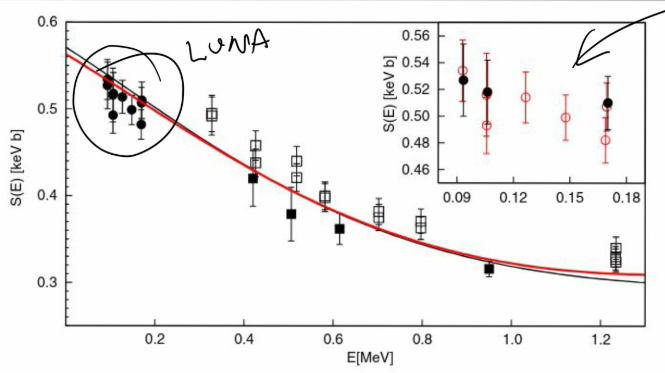
\includegraphics[scale=0.7]{Immagini/0415_SE2.png}
	\caption{Risultati di LUNA II. I quadratini pieni sono i dati vecchi, quelli vuoti sono i dati nuovi e i cerchi sono i dati di LUNA. Quelli nel riguadro in alto a sinistra sono in nero i dati con il metodo 2. e in rosso quelli con il metodo 1. (per LUNA non hanno discrepanza).}
	\label{0415_lunaii}
\end{figure}

\subsubsection{LUNA MV}\esperimento{LUNA!LUNA MV}
L'ultima frontiera per LUNA è una macchina acceleratrice con un voltaggio di $3.5$ MV detta appunto LUNA MV, ma per tale scopo le dimensioni non sono conformi allo spazio disponibile nei LNGS per cui verrà costruita da un'altra parte e questo lascia a disposizione LUNA II per possibili misurazioni future. L'obiettivo di LUNA MV sarà lo studio di reazioni di difficile misura e importanti per la verifica del modello; per esempio il cosidetto \textit{holy grail} dell'astrofisica\index{Holy Grail dell'astrofisica@\textit{Holy Grail} dell'astrofisica}\footnote{Guarda sezione \secrif{sec-holy-grail}.}:
$$\ce{^{12}C(\alpha,\gamma)\ce{^{16}O}}$$
Determinare la sezione d'urto di questa reazione permetterebbe di stimare le abbondanze di $\ce{^{12}C}$ e $\ce{^{16}O}$, difficili da misurare.

\paragraph{ATOMKI \textit{Anomaly}}\index{ATOMKI Anomaly@ATOMKI \textit{Anomaly}} Per quanto riguarda la ricerca di nuova fisica acceleratori di maggiore potenza permetterebbero lo studio dell'anomalia di ATOMKI\esperimento{ATOMKI}, per la prima volta osservata con la reazione
$$p+ \ce{^7Li} \to \ce{^8Be}^* \to \ce{^8Be} + \gamma^* $$
$$\ce{^8Be}\to \alpha + \alpha \qquad\quad \gamma^* \to e^+ + e^-$$
Non fecero \textit{particles identification}, ovvero non misurarono direttamente gli elettroni e i positroni prodotti. L'anomalia che osservarono fu un picco nella sezione d'urto per un angolo $\theta_{ee} \sim 120^{\circ}$; si è quindi pensato alla possibilità che venisse prodotta una particella massiva sconosciuta\footnote{Tipicamente le particelle della coppia hanno un angolo molto \vir{piccolo}.} (materia oscura) $\ce{^8Be}^* \to \ce{^8Be} + X$ e $X\to e^+ + e^- $ con $M_X\sim 17$ MeV, da cui il nome di particella X17\index{particella X17}.
Ci fu molta discussione al riguardo, anche perché il \textit{background} non era stato calcolato bene e non si era considerata la velocità di decadimento del $\ce{^8Be}$ in $2\alpha$.\\
ATOMKI si spinse più avanti\footnote{Anche nell'esperimento DAMA\esperimento{DAMA} ai LNGS dicono di aver osservato fluttuazioni di materia oscura, tuttavia solo loro riescono a ossevarle.} studiando:
$$p+\ce{^3H} \to \ce{^4He}+e^++e^-$$
Oltre al canale $\to \ce{^4He} +\gamma^*$ si potrebbe avere $\to \ce{^4He} + X$; osservarono la stessa anomalia. Questa reazione si può studiare con un metodo \textit{ab-initio}\index{Metodo ab-initio@Metodo \textit{ab-initio}} che ha confermato l'assenza di questo picco.\\
LUNA MV potrebbe mettere fine a questa discussione poiché riuscirà a raggiungere i 17 MeV per le reazioni $p+\ce{^3H}$ e $p+\ce{^7Li}$. Per quanto riguarda quest'ultima, sta per essere studiata al \textit{Laboratory of Paul Scherrer Institute} (LPSI) in Svizzera, dove cercano anche di misurare il decadimento non standard del $\mu$.

\subsection{ERNA}\esperimento{ERNA}
Un altro esperimento che discuteremo è \textit{European Recoil separator for Nuclear Astrophysics} o ERNA, situato a Caserta in Campania, che utilizza appunto il metodo del \textit{recoil} (adottato anche in altri esperimenti).

\subsubsection{\textit{Recoil mass separator}}
Studiamo la reazione poco probabile $a+b \to c+\gamma$ con $a$ ioni accelerati e $b$ targhetta, per esempio:
$$\ce{^4He} + \ce{^{12}C}\to \ce{^{16} O}+\gamma$$
Oltre alla radiazione che viene raccolta da un rilevatore, dal momento che la reazione è \vir{rara}, avremo un fascio uscente di $a$ e $c$; per separare il reagente dal prodotto si utilizza una macchina \textit{recoil mass separator}\index{recoil mass separator@\textit{recoil mass separator}} che sfrutta la differenza di massa tra $a$ e $c$ per deviare la traiettoria del fascio di $a$ attraverso campi magnetici, facendo sì che solo il fascio di $c$ raggiunga il rivelatore. Quest'ultimo è messo in coincidenza con il rivelatore di fotoni.

\subsubsection{Cinematica Inversa} 
Poniamoci nel sistema del centro di massa\footnote{Mettiamo $c=1$ e indichiamo le quantità riferite al sistema del centro di massa con l'apostrofo $'$.}, dove vediamo $a$ e $b$ scontrarsi e $\gamma$ e $c$ \vir{\textit{scatterare}} con un certo angolo $\theta_{CM}$:
\begin{align*}
	\text{Stato  }&\text{Iniziale} & \text{Stato  }&\text{Finale} \\
	(E_a',p',0,0) +&(E_b',-p',0,0) & (E_c',-p_c'\cos{\theta_{CM}},-p_c'\sin{\theta_{CM},0}) +&(E_\gamma',E_\gamma'\cos{\theta_{CM}},E_\gamma'\sin{\theta_{CM}},0) 
\end{align*}
Dalla conservazione del quadrimpulso:
\begin{align*}
	m_a+m_b + \underbrace{\frac{p'^{2}}{2\mu_{ab}}}_{T_{rel}} &= m_c + \cancel{\frac{E_\gamma'^2}{2m_c}}+E_\gamma' \\ 
	-p_c'\cos{\theta_{CM}} +& E_\gamma' \cos{\theta_{CM}} = 0\\
	-p_c'\sin{\theta_{CM}} +& E_\gamma' \sin{\theta_{CM}} = 0
\end{align*}
per cui $E_\gamma' = p_c'$ e $E_\gamma' = \overbrace{m_a+m_b-m_c}^{\Delta M} + T_{rel}$.\\ 
Nel sistema del laboratorio:
\begin{align*}
	\text{Stato  }&\text{Iniziale} & \text{Stato  }&\text{Finale} \\
	(E_a,p_a,0,0) +&(m_b,0,0,0) & (E_c,p_c\cos{\theta_{c}},p_c\sin{\theta_{c},0}) +&(E_\gamma,E_\gamma\cos{\theta_{\gamma}},E_\gamma\sin{\theta_{\gamma}},0) 
\end{align*}
da cui $p_{CM} =p_a$ ed $E_{CM} = m_b + E_a$; trasformando con Lorentz ($\beta = p_{CM}/E_{CM}$ e $\gamma = (1-\beta^2)^{-1/2}$) si ottiene:
$$p_{c,y} = p_{c,y}' \:\Rightarrow\: \tan{\theta_c} = -\frac{p_c' \sin{\theta_{CM}}}{\gamma [\beta E_c' +p_c'\cos{\theta_{CM}}]}$$
Ci chiediamo allora quale sia l'angolo massimo di scattering per $c$: $\sin{\theta_{CM}}=1$ per cui $\theta_{CM} = \pi/2$.
$$\tan{\theta_c}|_{\max{}} = \frac{p_c'}{\gamma\beta E_c'} = \frac{E_\gamma'}{\beta E_c}\simeq \frac{E_\gamma}{p_c} $$
dove abbiamo trascurato il segno e usato le trasformazioni di Lorentz nel secondo passaggio. Abbiamo allora che la traiettoria di $c$ sta dentro un cono di ampiezza massima $\theta_{c,\max{}} \sim \tan^{-1}{E_\gamma/p_c}$ e per convergere il fascio bisogna massimizzare $p_c$; questo scala come $p_{CM}$ che è maggiore per $m_a>m_b$.\\
Dunque, nello studio di $\ce{^4He} + \ce{^{12}C}$ si usa il carbonio come proiettile e non l'elio. Questa configurazione viene detta \textbf{cinematica inversa}\index{cinematica inversa} e migliora la separazione nella macchina di \textit{recoil}. Riportiamo uno schema dell'apparato sperimentale in Figura \ref{0415_schema}.\\
L'unico difetto del metodo sta nel fatto che minore è l'energia incidente maggiore dev'essere il raggio %! Raggio? Nel senso la lunghezza
della struttura.
\begin{figure}[!h]
	\centering
	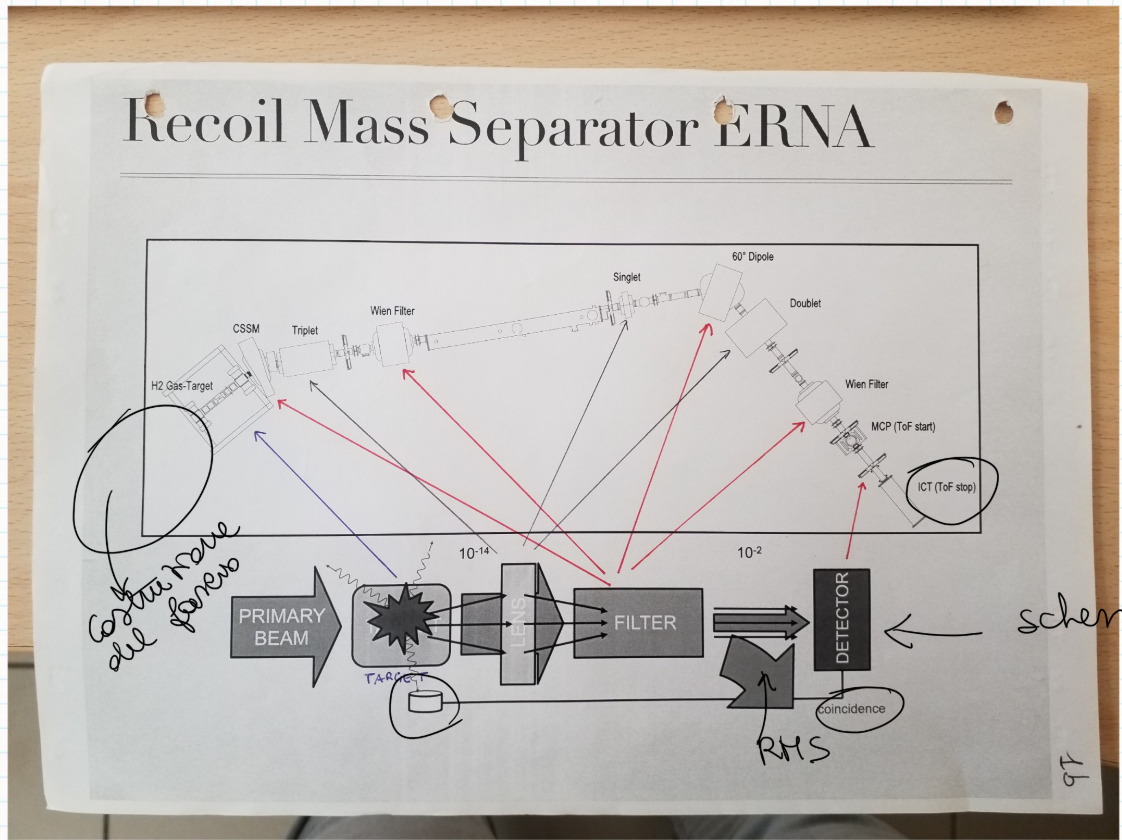
\includegraphics[scale=0.5]{Immagini/0415_schema.png}
	\caption{Schema dell'apparato sperimentale di ERNA: sono presenti lenti focalizzanti all'uscita di ogni filtro. In questo caso a curvare sono le $c$ mentre le $a$ vanno a dritto.}
	\label{0415_schema}
\end{figure}







